\documentclass[12pt]{article}
\PassOptionsToPackage{quiet}{fontspec}
\usepackage[a4paper, total={6.5in, 10in}]{geometry}
\usepackage{amsmath}
\usepackage{mathtools}
\usepackage{amsfonts}
\usepackage{mathrsfs}
\usepackage{bm}
\usepackage{enumerate}
\usepackage{tikz}
\usepackage{ctex}
\usepackage{pgfplots}
\pgfplotsset{compat=1.17}
\usepackage{xcolor}
\usepackage{float}
\usepackage{booktabs}
\usepackage{graphicx}
\usepackage{framed}

\title{}
\date{\today}
\author{}

\begin{document}
    
    \begin{titlepage}
        \centering
        \vspace{0.2\textheight}  
        {\huge 神经网络python编程}
        \vspace{0.025\textheight}
        \vspace{0.1\textheight}

        {\Large ZongPingD}
        \vfill 
        {\large \today}
        \vspace{0.1\textheight} 
    \end{titlepage}
    \tableofcontents
    \newpage

    \section{神经网络工作原理}
    \subsection{预测器}
    设有函数关系式$y=f(x,\xi)$,其中$y_i$为真实值,y为预测值。
    核心思想:使用误差,在不知道确切的函数关系时,根据已知数据计算误差,然后通过调整参数$\xi$来减小误差;
    第i次调整后的参数值记作$\xi_{i}$使用这种方法是因为很多的问题都无法用简单的函数关系来刻画。如图即为一
    个预测器的模型.
    
    误差值的计算方法为:误差 = 期望目标值-(带入参数后的)估计值
    \begin{figure}[!htb]
        \centering
        % 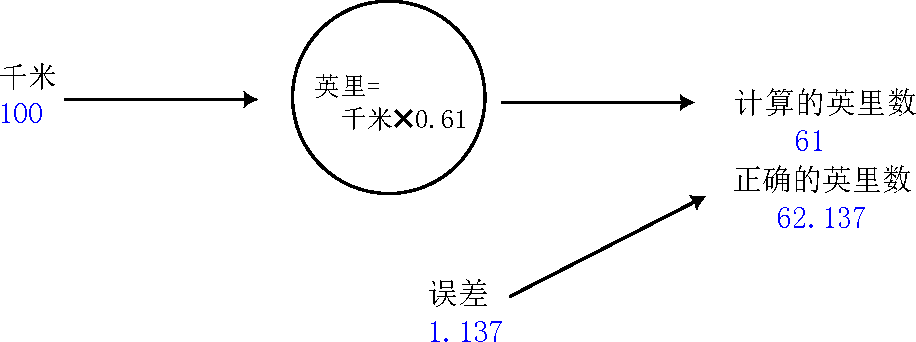
\includegraphics[scale=0.5]{./picture/pic1.pdf}
        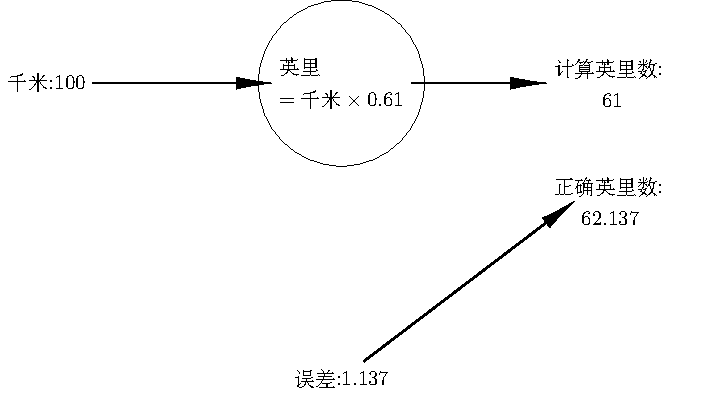
\includegraphics[scale=1]{./picture/gapsGenerate.pdf}
    \end{figure}
    \vspace{1em}

    \begin{equation}
         E = f(x,\xi_{i})-y_{i}
    \end{equation}

    \vspace{1em}
    细化误差值:如果输出值越来越接近正确答案,即误差值越来越小,
    那么我们就不要做那么大的调整。使用这种方式,我们就可以避免像先前那样得到超调的结果,即:
    \begin{equation}
        |f(x,\xi_{i+1})-y_i|>|f(x,\xi_{i})-y_i|
    \end{equation}
    我们尝试得到一个答案,然后使用误差不断地进行修正,也就是\textbf{迭代}

    \subsection{分类器}
    声明:预测器于分类器并没有多大的区别。

    关键:找到参数$\xi$与误差的关系,而我们的参数$\xi$的初始值是一个随机值。
    然后得出$\Delta \xi=g(E,x)$,即x改变多少可以使得参数$\xi=\xi_{i}+\Delta\xi_i$的值比骄合适,
    能够达到划分的目的。其中的$\xi_{i}$为每次修正后的值。把每个数据都训练一遍,如果有n个数据,那么就训练n次,
    最终的$\xi=\xi_{n}$.

    数据才是判断标准!!!
    
    但是这样的训练仍然是由很大的问题的:实际上,最终改进的直线不会顾及所有先前的训练样本,
    而是抛弃了所有先前训练样本的学习结果,只是对最近的一个实例进行了学习。为改善这种情况我们只采用$\Delta E$
    的几分之一,这样就能够保留原本的训练结果的同时又加入了新的训练结果,类似于MA模型。这个“几分之几”的比例,
    我们称为学习率,记作L,有如下的关系:
    \begin{equation}
        \Delta \xi' =L(\Delta \xi)
    \end{equation}
    这样的好处:规避错误的训练数据或者是噪声,放置了单次的学习数据主导了整个的学习过程

    \subsection{多个分类器}
    比如下边的这个抑或函数XOR(x,y)的作用就无法使用直线刻画,表现在图上就是不能用直线进行分类器的构造。
    % \begin{figure}[!htb]
    %     \centering
    %     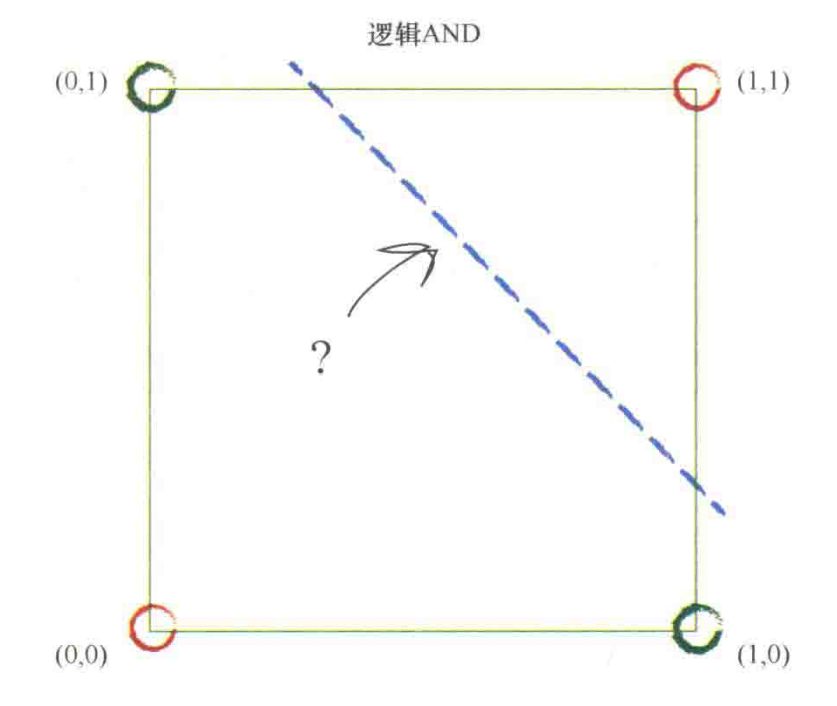
\includegraphics[scale=0.5]{picture/异或函数.png}
    % \end{figure}
    也就是说一个简单的线性分类器无法学习到XOR(x,y)这个函数。
    为此我们使用两个线性分类器进行划分,多个线性分类器就可以分割出异性区域,这就是神经网络的核心思想.
    两个线性规划器的划分结果如下:

    \begin{figure}[!htb]
        \centering
        % 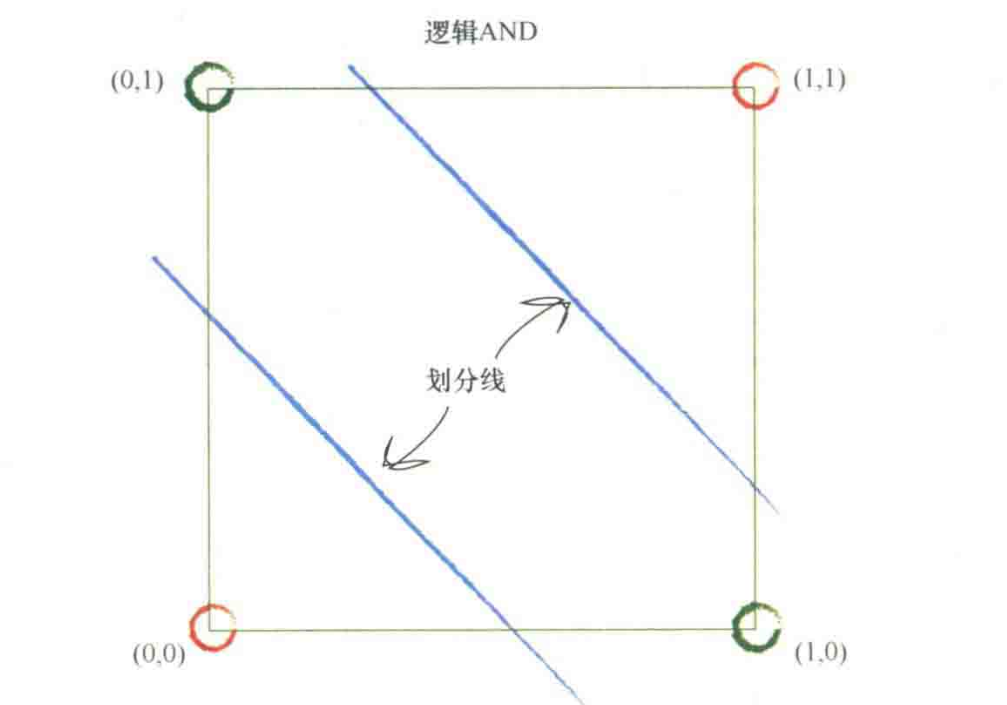
\includegraphics[scale=0.4]{picture/神经网络雏形.png}
        % 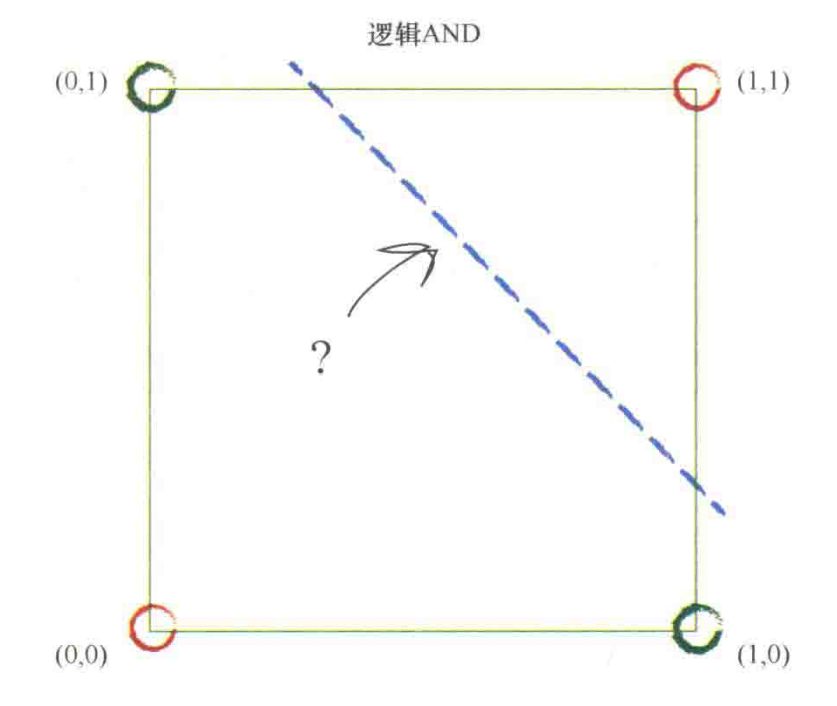
\includegraphics[scale=0.4]{picture/异或函数.png}
        \leavevmode\lower1em\hbox{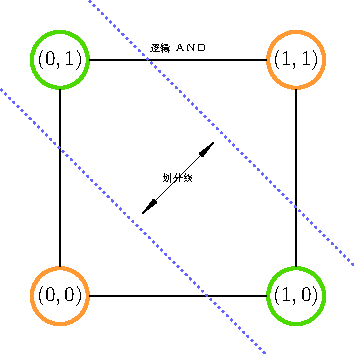
\includegraphics[scale=1]{picture/Classfication1.pdf}}
        \hspace*{4em}
        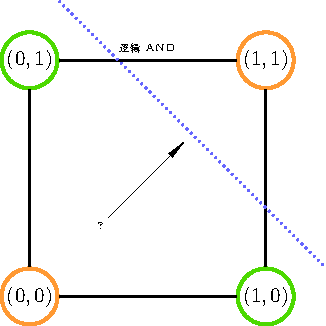
\includegraphics[scale=1]{picture/Classfication2.pdf}
    \end{figure}

    \subsection{神经元}
    生物的多个神经元组合在一起可以完成非常复杂的生物生理活动。
    但是单独的一个神经元我们不能够简单的看作一个线性函数:即输出=(某个常数$\times$输入-某个常数)。
    观察表明,神经元不会立即反应,而是会抑制输入,直到输入增强,强大到可以触发输出。你可以这样认为,
    在产生输出之前,输入必须到达一个阈值(threshol)。也就是激活函数,又叫做S函数,
    主要又两类的激活函数,如图:
    \begin{figure}[!htb]
        \centering
        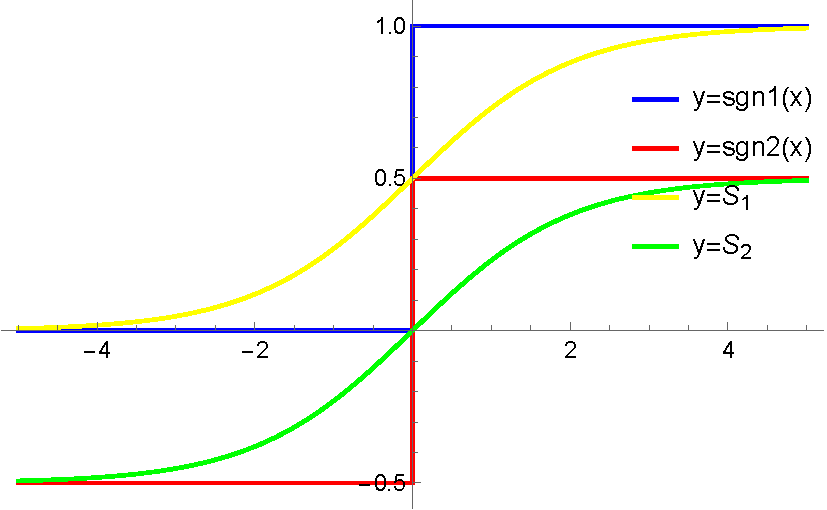
\includegraphics[scale=0.5]{./picture/激活函数.pdf}
        \label{两种类型的激活函数}
        \caption{两种类型的激活函数两种类型的激活函数:阶梯函数,sigmoid函数}
    \end{figure}

    对神经元建模主要需要考虑如下的问题, 由此便产生了神经网络:
    \begin{itemize}
        \item 一个神经元可以接受多个的输入,对多个输入相加即的总和
        \item 总和足够大的达到激活函数的标准情况下,才会产生输出信号
        \item 一个神经元可以传到下一层的多个神经元
    \end{itemize} 


    \subsection{神经网络中的信号追踪}
    神经网络第一层节点仅仅只是输入层,只有输入功能,不必应用输入函数
    下边的讨论基于一个三层的神经网络;
    中间层第$i$个节点的输入值等于第一层的所有的节点输出到该点的加权平均,记作$\sum\limits_{i}$,
    于是乎节点$i$的输出为$\frac{1}{1+e^{-\sum_i}}$.
    由此即可计算出中间层的每个节点$i$的输出,第三层的输出计算方法同理.
    但是神经网络的层数一旦过多计算量就会猛然增加,于是乎引入矩阵的乘法进行输入的计算

    \subsection{神经里的矩阵乘法}
    \begin{figure}[!htb]
        \centering
        % 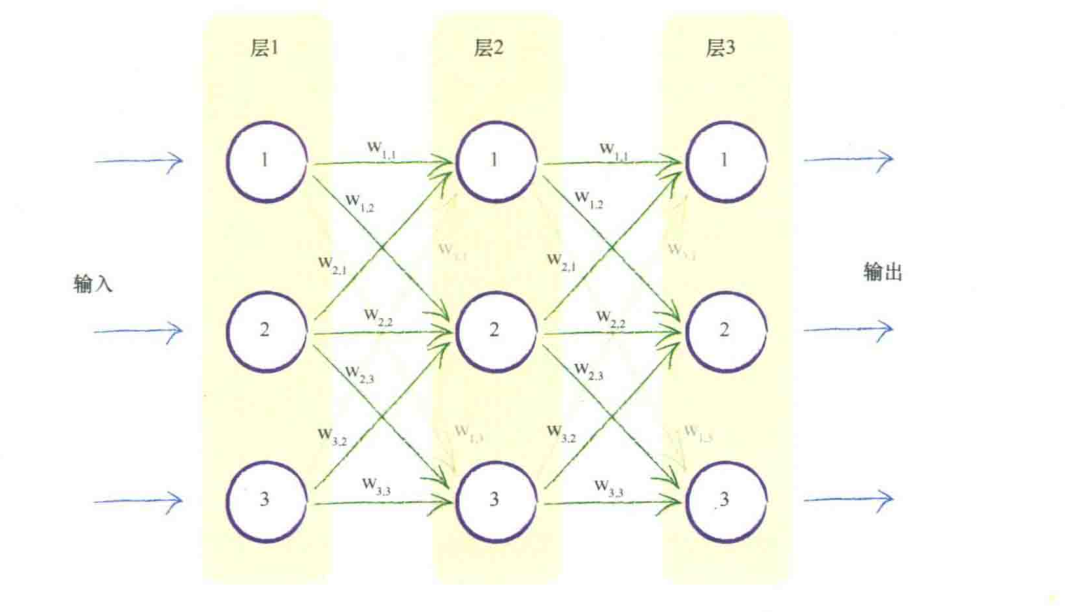
\includegraphics[scale=0.5]{./picture/神经网络.png}
        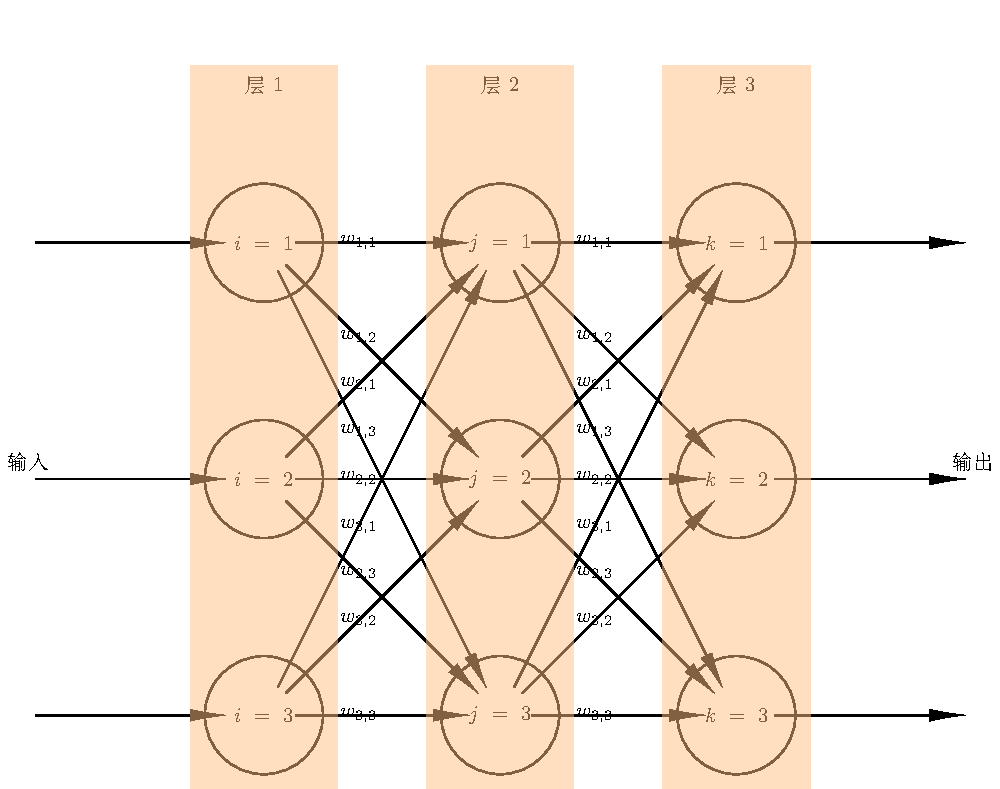
\includegraphics[scale=0.5]{./picture/MatrixProd.pdf}
    \end{figure}
    中间层的节点的输入值等于第一层的所有的节点的加权平均,对于隐藏层的第i个节点,假如:
    输入层的输入向量为
    \[
        v_1=
        \begin{bmatrix}
        a_11\\
        a_21\\
        a_31 
        \end{bmatrix}
    \]

    设节点$i$到节点$j$的权重为$w_{ij}$
    那么有计算可知
    \begin{equation}
        \sum_i=a_1w_{1i}+a_2w_{2i}+a_3w_{3i}
    \end{equation} 

    设中间层有$n$个节点,我们可以
    \begin{equation}
        \sum_{i}=\sum_{j=1}^{n}{a_jw_{ji}}    
    \end{equation}

    把以上中间层的所有神经元考虑进来,记中间层的输出向量为
    $$
    v_2=
    \begin{bmatrix}
        a_{12}\\
        a_{22}\\
        \vdots\\
        a_{33} 
    \end{bmatrix}
    $$

    可以得到这相邻的两层之间的转移矩阵表达式为
    \begin{equation}
        v_2
        =
        \begin{bmatrix}
             w_{11} & w_{21} & \cdots & w_{n1}\\
             w_{12} & w_{22} & \cdots & w_{n2}\\
             \cdots\\
             w_{1n} & w_{2n} & \cdots & w_{nn}\\
        \end{bmatrix} 
        \begin{bmatrix}
            a_11\\
            a_21\\
            \vdots\\
            a_n1 
        \end{bmatrix}
    \end{equation}

    这一过程记作$O={\rm sigmoid}(X)$, $O$代表中间层输出,$X$为上一层的输出,
    $f(x)={\rm sigmoid}(x)$中的$f(x)$本质就是一个激活函数,常取$\frac{1}{1+e^{-x}}$,
    而隐藏层和输出层之间之间的转移矩阵记为$w_{\rm hidden\_output}$,
    所以隐藏层的输出为$O_{\rm hidden}={\rm sigmoid}(X_{\rm hidden})$。

    \subsection{多层神经网络中的权重调整}
    \subsubsection{单个输出节点}
    本质还是类似于之前的分类器,计算出误差值,然后根据误差值去调整权重。
    但是如果使用计算出来的误差只对单独的一个权重进行调整是不合理的,因为只有一条链接造成误差的概率是非常小的,
    所以我们会尽量的调整多个权重。
    如何把误差应用到权重的调整上呢?我们有如下的两种做法:
    \begin{itemize}
        \item 等分误差
        \item 不等分误差,权为前一层所有节点对应到节点$i$的权重
    \end{itemize}
    这一思想称为{\textcolor{red}{误差的反向传播}}\\
    输出层有多个节点时,每个节点的误差反向传播和之前类似,这是因为进入输出节点的链接不依赖于另一输出节点的链接
    也就是对于不同输出节点的两组链接之间不存在依赖关系

    \subsubsection{多个输出节点}
    设隐藏层的前一层有$n$个节点,隐藏层的节点$i$反向传播后的$w_{ji}$变为
    \begin{equation}
        w'_{ij}=\frac{w_{ij}}{\sum_{j=1}^{n}{w_{ji}}}
    \end{equation}
    如图所示即为$w'_{ij}$的图解意义:
    \begin{figure}[!htb]
        \centering
        % 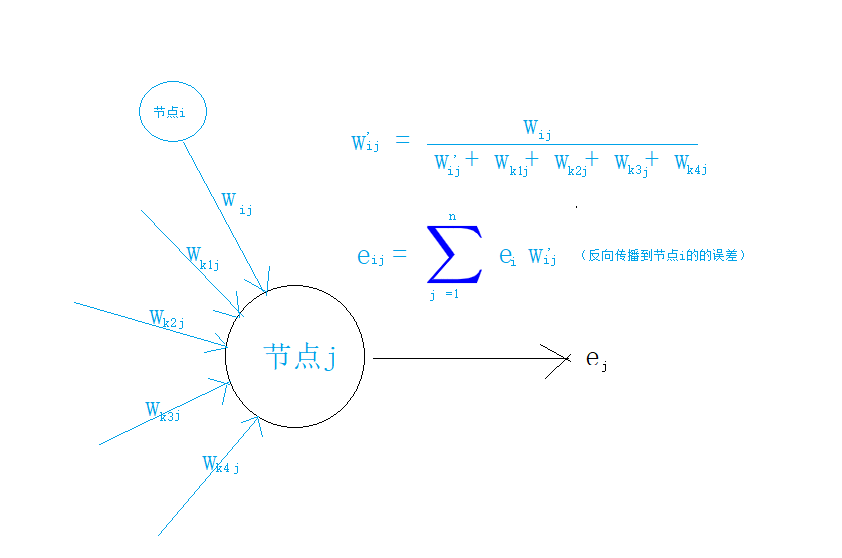
\includegraphics[scale=0.5]{picture/误差反向传播矩阵.png}
        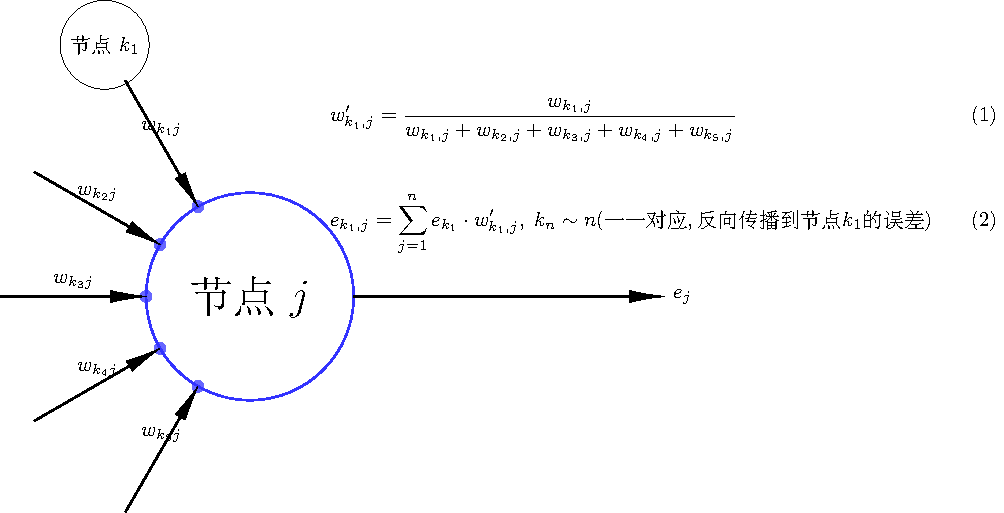
\includegraphics[scale=0.5]{picture/InverseBoardCast.pdf}
    \end{figure}
    所以$w'_{ij}$可以看作是节点$j$对于节点$i$的反馈度
    \subsubsection{原理神经网络输出层的权重调整}
    我们将输出误差标记为$e_{\rm output}$,与隐藏层相关的误差记作$e_{\rm hidden}$,
    输出层和隐藏层之间的链接权重记为$w_{\rm ho}$,输入层与隐藏层之间的链接权重记为$w_{\rm ih}$
    现在的重点记为中间层的误差计算,但是中间层并没有明显的误差,因为我们没有目标值与希望输出的值。
    我们的训练数据给出了我们最终的节点目标值,并没有给出中间层的目标值,所以对此我们的方法就是
    从输出层实施反向传播进行误差重组,进而计算出之前的每一层的误差。
    记隐藏层的节点$i$的误差为$e_{\rm hidden\_i}$,设输出层有$n$个节点,那么我们就有
    \begin{equation}
        e_{{i}_{\rm hidden}}=
        \sum_{j=1}^{n}{e_{{ji}_{\rm output}}w'_{{ji}_{\rm ho}}}
        \label{ei误差}
    \end{equation}
    相关的图示为
    \begin{figure}[!htb]
        \centering
        % 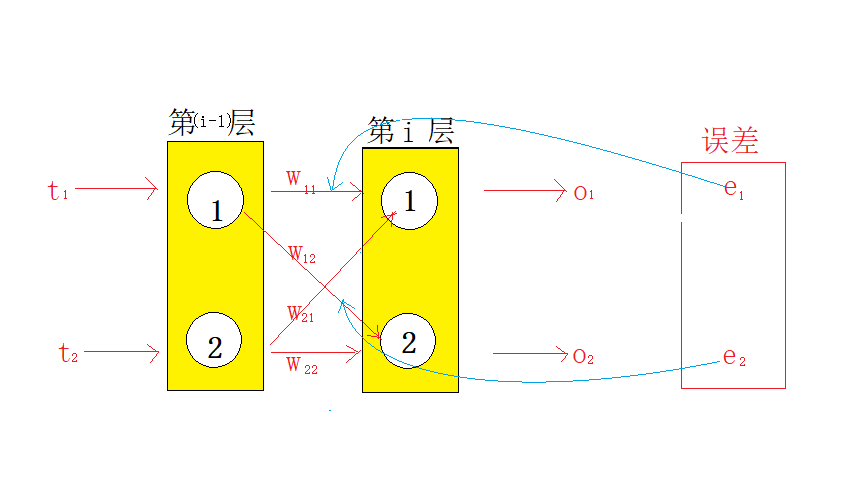
\includegraphics[scale=0.5]{picture/误差反向传播.png}
        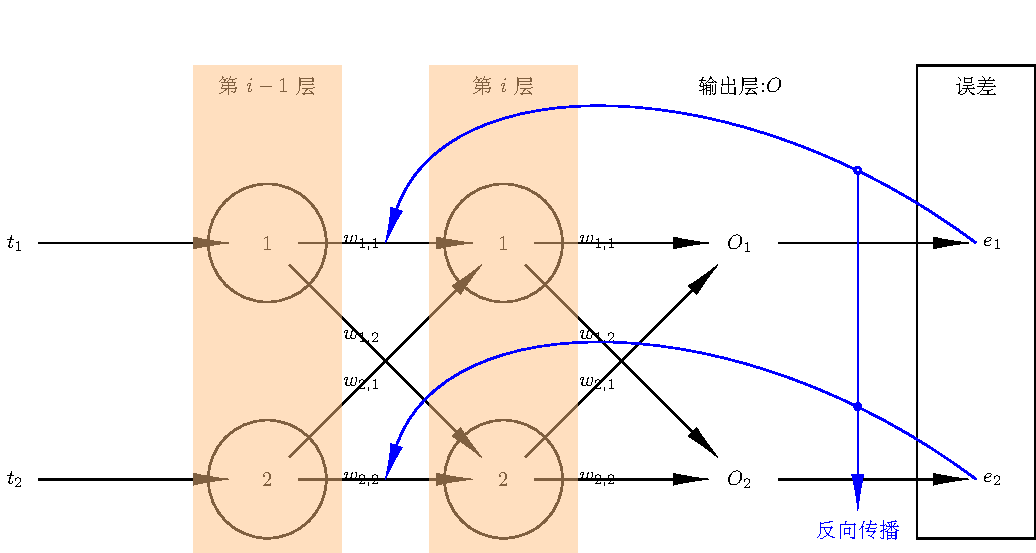
\includegraphics[scale=0.5]{picture/gapsDistrio.pdf}
    \end{figure}
    注意:在权分误差时,所有的权重来自于连接在同一个已知误差的节点
    \subsubsection{使用矩阵进行反向误差传播}
    首先可以知道隐藏层的节点i的误差$e_{{i}_{\rm hidden}}=\sum_{j=1}^{n}{e_jw'_{{ij}_{\rm ho}}}$,
    记$z_{ij}=w'_{ij}$,记我们的中间层i的误差为
    \begin{equation}
        Error_{{i}_{\rm hidden}}
        =
        \begin{bmatrix}
            e_{i,1}\\
            e_{i,2}\\
            \vdots\\
            e_{i,n}
        \end{bmatrix} 
    \end{equation}
    那么我们可以得到,误差计算的矩阵形式为:
    \begin{equation}
        Error_{\rm hidden}=
        \begin{bmatrix}
            z_{11} & z_{12} & \cdots & z_{1n}\\
            z_{21} & z_{22} & \cdots & z_{2n}\\
            \vdots\\
            z_{n1} & z_{12} & \cdots & z_{nn}\\
        \end{bmatrix}
        \begin{bmatrix}
            e_{i+1,1}\\
            e_{i+1,2}\\
            \vdots\\
            e_{i+1,n}
        \end{bmatrix}
    \end{equation}
    但是这种形式过于复杂,但是我们可以从上面的矩阵可以看出,矩阵每个元素的就相当于是进行了归一化处理。
    较大的比例仅仅是代表误差对于隐藏层的影响较大而已,所以我们直接去掉每个元素的分母,这样我们仅仅只是
    失去了后馈误差的大小,并没有失去它在对于中间层节点i的整个误差中的所占比例。所以我们就采用这样一个
    比较简单的形式替代原来的矩阵。这种把归一化因子除去的与原来复杂的形式相比是一样有效的。因为反馈过大
    或者是过小,在下一轮的学习中,神经网络是能够进行自我更正的,此时的误差计算矩阵等于
    \begin{equation}
        Error_{\rm hidden} =
        \begin{bmatrix}
            w_{11} & w_{12} & \cdots & w_{1n}\\
            w_{21} & w_{22} & \cdots & w_{2n}\\
            \vdots\\
            w_{n1} & w_{12} & \cdots & w_{nn}\\
        \end{bmatrix}
    \end{equation}

    可以看出,这个矩阵就是之前矩阵乘法里边的那个转移矩阵的转置.
    
    \textbf{转置原因:}
    {\kaishu 因为原来的那个矩阵是前一层的所有节点的加权平均,而后边的误差转移矩阵式后一层的加权平均。}

    \subsection{更新权重}
    \subsubsection{问题背景}
    在前面我们已经让误差传递到了神经网络的每一层,下边自然就是解决,神经网络中的权重的更新了。
    精准的计算输出的表达式如下\\
    这是一个简单的3层、每层3个节点的神经网络,其中输入层节点的输出是输入值和链接权重的函数。
    在节点$i$处的输入是
    $x_i$, 连接输入层节点$i$到隐藏层节点$j$的链接权重为$w_{i,j}$,
    类似地,隐藏层节点$j$的输出是$x_j$,连接隐藏层节点$\mathrm{j}$  
    和输出层节点$k$的链接权重是$w_{j,k}$
    \begin{equation}
        O_{k}=
        \frac{1}{1+e^{-\sum_{j=1}^{3}{[w_{j, k}\cdot 
        \frac{1}{1+e^{-\sum_{i=1}^{3}\left(w_{i, j} x_{i}\right)}}
        ]}}}
        \label{Output}
    \end{equation}
    明显可以看出很难从方程\refeq{Output}中得到误差与权重的关系,而且即使能够计算出来他们的关系,
    我们训练这个模型也会花费十分漫长的时间。
    \subsubsection{梯度下降法}
    为此我们需要引进\textbf{梯度下降法}\\
    引入梯度下降法的原因:从上边得出我们的误差函数$O(x)$太过于复杂,所以我们无法从全局的观点下处理这个复杂的函数,
    得到精确的结果,但是我们可以使用梯度下降法从局部出发,只要我们每次"下降"一小步,但是我们的每个一小步都是”最优“
    的,那么我们可以知道我们的最终结果也是接近最优的。类似于算法里边的动态规划思想。

    一维坐标下边的梯度方向实际上就是x的正或负半轴,但是在二元函数里边,就不止x轴这两个方向了,
    可以看作是$360^{\circ}$,每个角度都对应这一个方向,角度由方向余弦决定。
    如图所示;
    \begin{figure}[!htb]
        \centering
        % 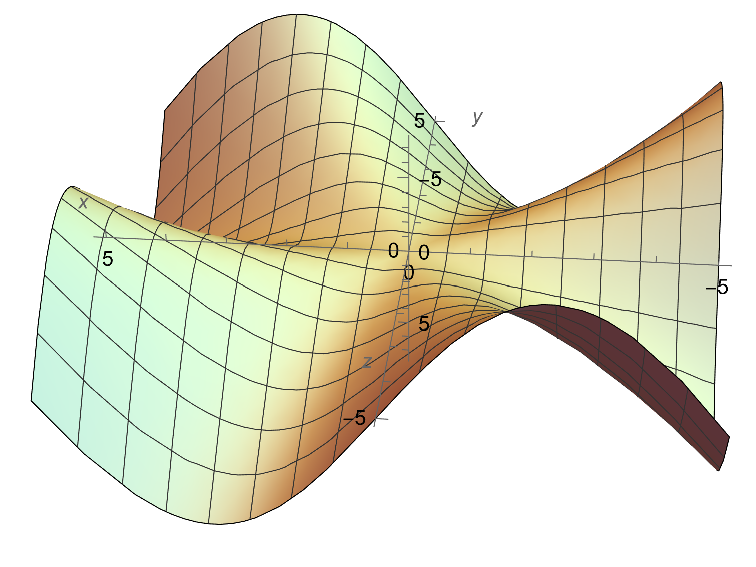
\includegraphics[scale=0.5]{./picture/梯度下降法.pdf}
        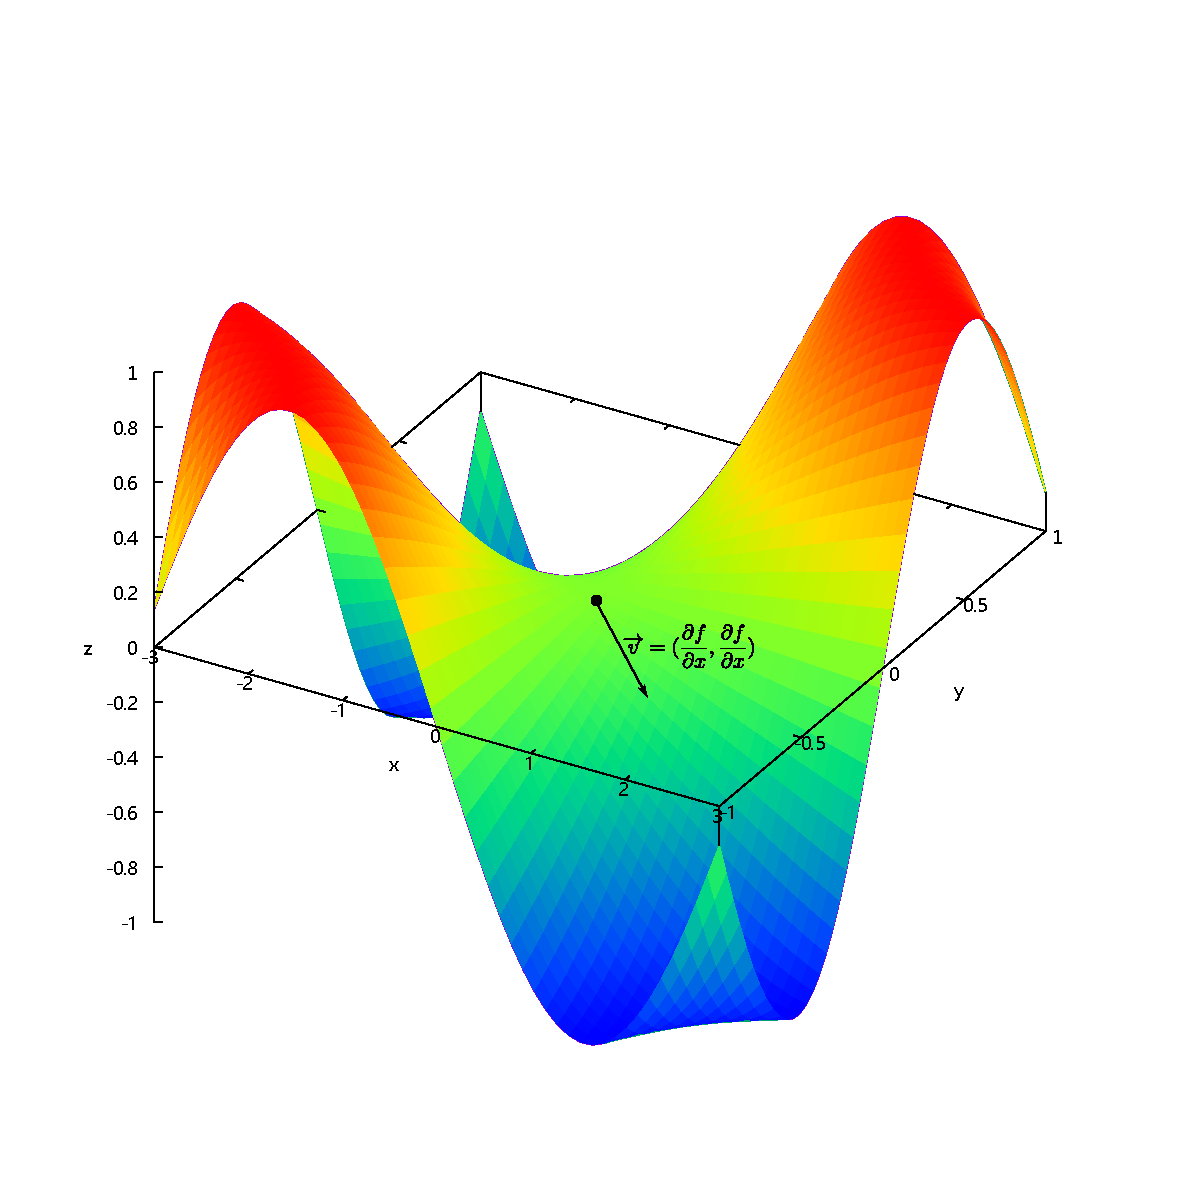
\includegraphics[scale=0.5]{./picture/Gratitude_Note.pdf}
        \label{梯度下降}
        \caption{梯度下降示意图($y=\sin(xy)$)}
    \end{figure}
    % 绘制图现象的GNuPlot代码
    % Terminal type is now 'qt'
    % Encoding set to 'default'.
    % gnuplot> f(x, y) = sin(x*y)
    % gnuplot> set xlabel "X"
    % gnuplot> set ylabel "Y"
    % gnuplot> unset key
    % gnuplot> splot f(x, y)
    % gnuplot> set xyplane at 0
    % gnuplot> set isosamples 50
    % gnuplot> set hidden3d
    % gnuplot> set pm3d
    % gnuplot> set palette
    % gnuplot> set palette rgbformulae 22, 13, -31
    % gnuplot> set xrange [-3:3]
    % gnuplot> set yrange [-1:1]
    % gnuplot> replot
    加入在原点,我们可以知道沿某些方向,函数值$z=f(x,y)$会增加;沿着某些方向,函数值会减小。
    所以必定会在某个方向增加的最快,在某个方向减小的最快,这个方向就是梯度的方向。也即向量
    $(f_x,f_y,f_z)$的方向。注意:在接近最小值的地方可以适当减小步长,远离最小值的地方可以适当的增大步长,
    防止出现超调的现象,我们可以近似的认为:步长正比于斜率。同时应该注意我们梯度下降法得到的是函数的最值,
    并不一定是极值。为了避免终止于错误的极值或错误的函数最小值,我们从定义域D内的不同点开始,
    多次训练神经网络,确保并不总是终止于错误的最值。不同的起始点意味着选择不同的起始参数,
    在神经网络的情况下,这意味着选择不同的起始链接权重。

    对于误差函数的选择有如下的几个备选项:
    \begin{itemize}
        \item 目标值-实际值
        \item |目标值-实际值|
        \item (目标值-实际值$)^2$
    \end{itemize}
    目标值就是训练数据,真实值就是网络的真是输出值。
    但是第一个方法会存在误差的正负抵消问题,第二个方法产生的误差函数在最小值附近不一定可导,
    所以我们选择第三种方法
    它只要有如下的优点
    \begin{itemize}
        \item 容易计算梯度下降的斜率
        \item 函数处处连续,可以很好的适合梯度下降法
        \item 由于可导,所以可以更加容易调整步长,防止出现超调
    \end{itemize}
    现在我们需要计算出\textbf{误差相对于权重的斜率}

    也就是说我们要计算的是,误差函数是如何依赖于神经网络中的链接权重的。
    这个问题的另一种表述方式为“误差对链接权重的改变有多敏感”
    一下即为一个权重与误差的对应关系图
    \begin{figure}[!htb]
        \centering
        % 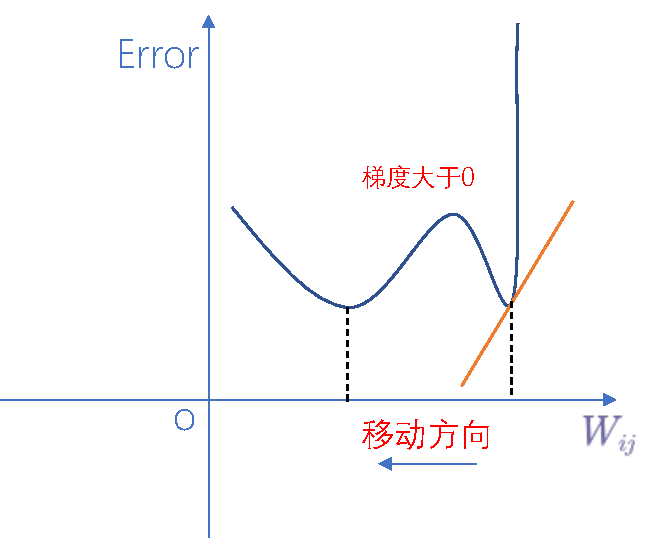
\includegraphics[scale=0.7]{picture/梯度下降.pdf}
        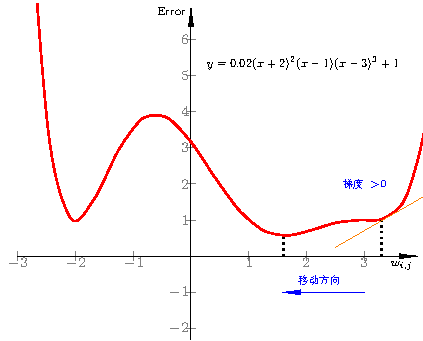
\includegraphics[scale=1]{picture/2dfun.pdf} 
        \caption{误差-权重关系图}     
        \label{误差-权重关系图}
    \end{figure}
    如果是误差相对与两个权重的关系图,那么这个图示就是一个三维的曲面,类似于图\ref{梯度下降}。
    如果是误差关于$n$个权重的关系时,梯度下降的思路还是相同的。
    \newpage
    \subsubsection{实际误差的理解}
    其实从上边可以看出,我们的结果往往是一个$n$维列向量,那么怎么从这个$n$维的列向量中找到误差了?

    我们有训练数据($n$个),这个就是目标值,输出的数据就是$n$个真实值,所以真实数据和目标数据是一一对应的,
    所以就会产生$n$个误差

    \subsubsection{计算公式推导}
    我们使用如下的三层神经网络进行推导,其他的神经网络推导相同。
    \begin{figure}[!htb]
        \centering
        % 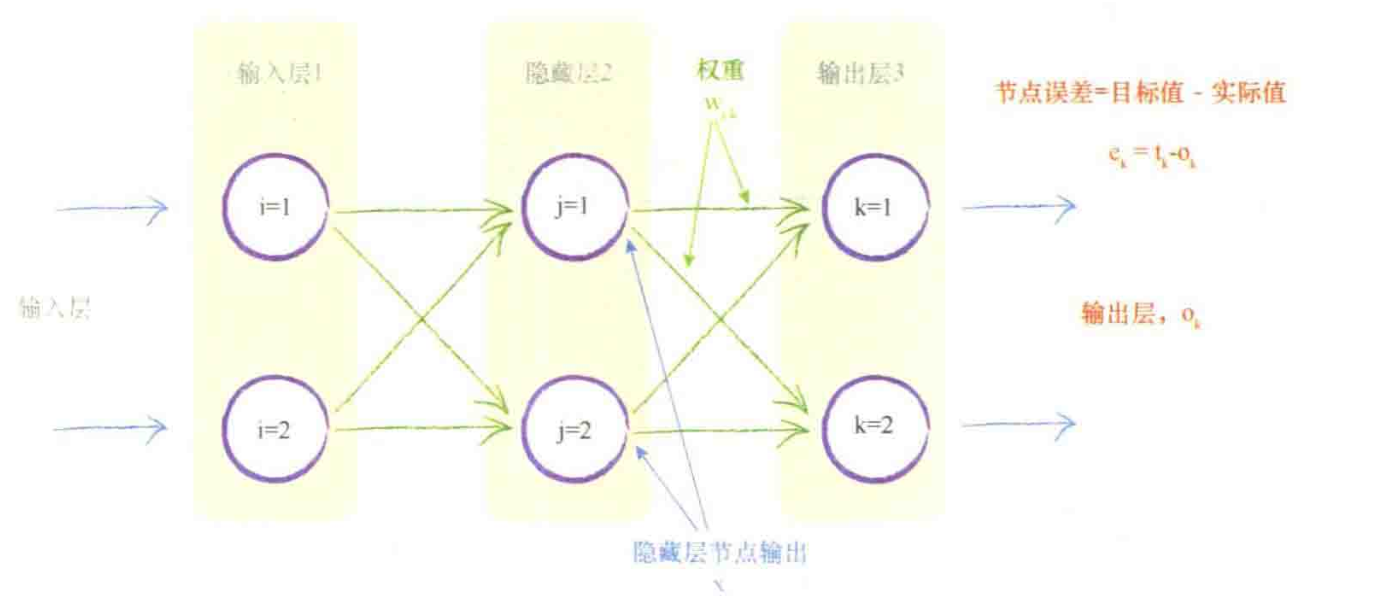
\includegraphics[scale=0.5]{picture/计算公式推导.png}  
        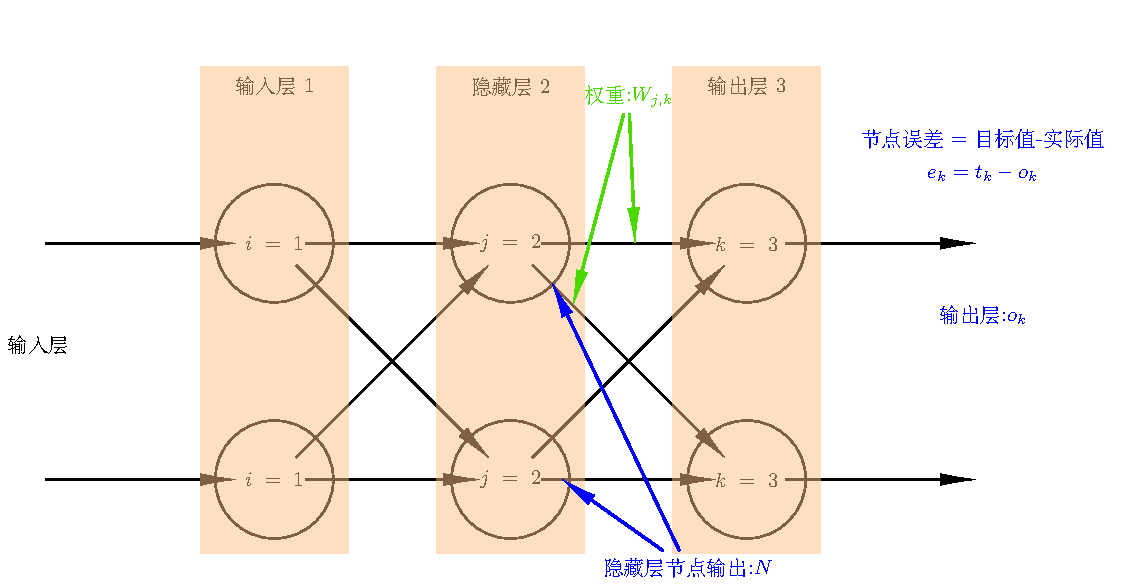
\includegraphics[scale=0.5]{./picture/Nueral_Net.pdf}    
    \end{figure}

   我们先研究误差对应一个权重的情况,记次权重为$w_{j,k}$,注意:这里的$j$代表上一层节点,$k$代表下一层节点
   误差关于次权重的变化率即为$\frac{\partial E}{\partial w_{j,k}}$, 于是我们有
   \begin{equation}
        \frac{\partial E}{\partial w_{j,k}} 
         = \frac{\partial}{\partial w_{j,k}}\left[\sum_{i=1}^{n}{(t_n-O_n)^2}\right]  
   \end{equation}

   注意到在节点$n$的输出$O_n$只与连接到这个节点的链接有关,即$O_k$只与$w_{j,k},\; j =(1, 2, 3,\cdots)$
   有关,所以我们可以在上边的和式中出去除$O_k$外的$O_n$,而且常数求导等于0,于是上边的表达式化简为
   \begin{equation}
    \frac{\partial E}{\partial w_{j,k}} 
     = \frac{\partial}{\partial w_{j,k}}{(t_k-O_k)^2}  \nonumber
    \end{equation}

    同时因为$O_k$是可以使用权重前置信号,也就是说$w_{j,k}$是关于$O_k$的函数,所以根据复合函数的微分法则,有
    \begin{align}
        \frac{\partial E}{\partial w_{j,k}} 
        & = \frac{\partial }{\partial w_{j,k}}{(t_k-O_k)^2}  \nonumber\\
        & = -2 (t_k-O_k)\cdot \frac{\partial O_k}{\partial w_{j,k}} \nonumber
    \end{align}
    又由前边可以知道$O_k$就是输入信号的加权求和激活,即
    \begin{equation}
        O_k={\rm sigmoid}\left(\sum_{j=1}^{n}{w_{j,k}\cdot O_j}\right)
        \nonumber
    \end{equation}
    这里的$O_j$就是前一隐藏层的节点输出,此时的sigmoid还可以进行微分,所以最终可以得到
    \begin{align}
        \frac{\partial E}{\partial w_{j,k}}
        & = -2 (t_k-O_k)\cdot {\rm sigmoid}\left(\sum_{j=1}^{n}{w_{j,k}\cdot O_j}\right)
        \cdot\left[1-{\rm sigmoid}\left(\sum_{j=1}^{n}{w_{j,k}\cdot O_j}\right)\right]
        \cdot \frac{\partial}{\partial w_{j,k}}{\left[\sum_{j=1}^{n}{w_{j,k}\cdot O_j}\right]}\nonumber\\
        & = -2 (t_k-O_k)\cdot {\color {red}{\rm sigmoid}(\sum_{j=1}^{n}{w_{j,k}\cdot O_j})}
        \cdot\left[1-{\color {red}{\rm sigmoid}(\sum_{j=1}^{n}{w_{j,k}\cdot O_j})}\right]
        \cdot O_j \nonumber\\
        & = -2(\mbox{目标值-实际值})\cdot {\rm sigmoid}(i'_k)\cdot [1-{\rm sigmoid}(i'_k)]\cdot O_j \nonumber\\
        & = -2(e_k)\cdot {\rm sigmoid}(i'_k)\cdot [1-{\rm sigmoid}(i'_k)]\cdot O_k
    \end{align}

    其中的$i'_k$即为最后一层($k$层)没用经过激活函数的输入信号,$e_k$就是隐藏层节点中重组的向后传播误差,
    $O_j$即为前一隐藏层节点$j$的输出(对比$O_k$),$O_k$为输出层的输出数据,与$O_j$没有在同一层.

    让我们把最后的结果拿出来,然后去掉误差前边的倍数2,这个就是我们要求的斜率表达式.
    \begin{framed}
        \begin{equation}
            % \boxed{\frac{\partial E}{\partial w_{j,k}}=-e_k\cdot {\rm sigmoid}(i'_k)\cdot [1-{\rm sigmoid}(i'_k)]\cdot O_k}
            \frac{\partial E}{\partial w_{j,k}}=-e_k\cdot {\rm sigmoid}(i'_k)\cdot [1-{\rm sigmoid}(i'_k)]\cdot O_k
            \label{输入层和隐藏层}
        \end{equation}
    \end{framed}

    \textbf{注:这里把输入记为$i'_k$的原因:经过激活函数处理的输入才是真正的输入}

    \subsubsection{梯度下降处理}
    经过上边的一番折腾,现在我们找到了误差函数,所以我们可以开始寻找误差函数的斜率(关于权重)了。进而进行梯度下降处理
    尽量找到一个权重使得误差尽可能的小,下边是各个参数的理解。
    \begin{figure}[!htb]
        \centering
        % 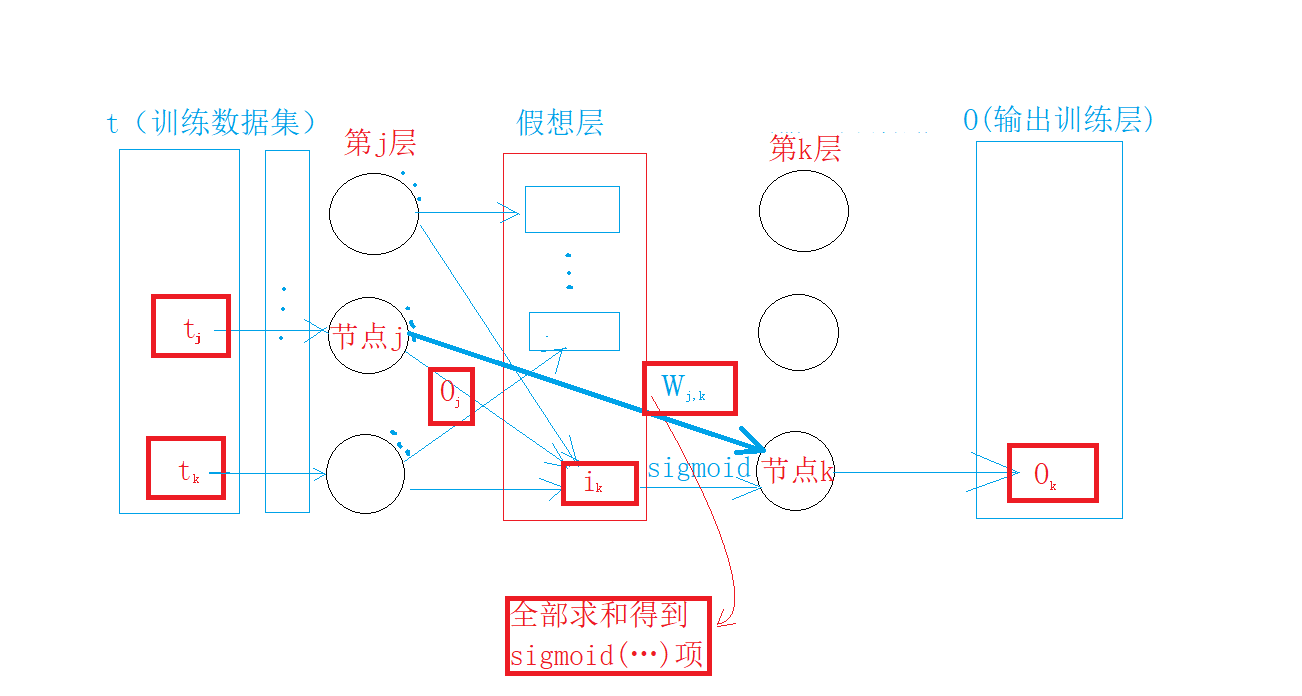
\includegraphics[scale=0.5]{picture/参数理解.png}
        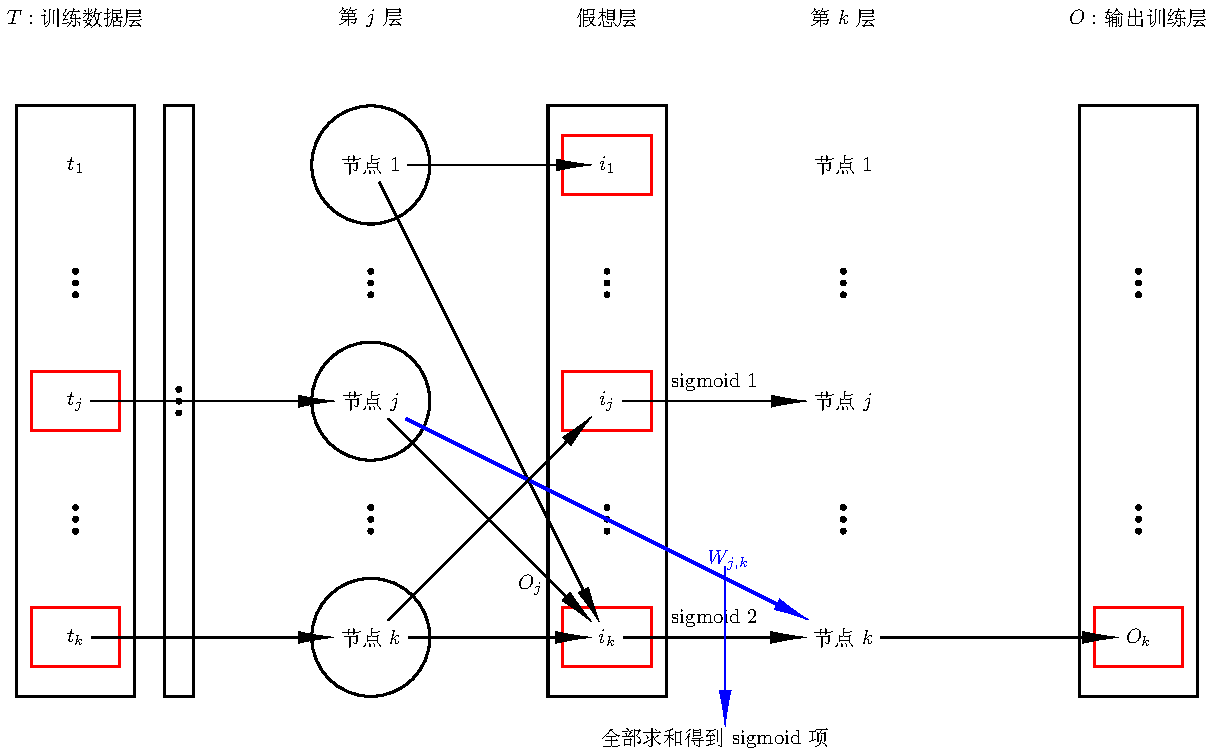
\includegraphics[scale=0.5]{picture/coef_init.pdf}
        \label{实际参数的分布}
        \caption{斜率方程参数的分布。注:$t_k$是与$O_k$水平的}
    \end{figure}

    \textbf{注:权重的方向与梯度的方向相反}


    现在我们已经解决了输出层和隐藏层之间的权重调整问题,接下来我们回去解决输入层和隐藏层之间的权重。
    与之前的求解方法类似,新权重集的表达式也是分为三个部分
    \begin{itemize}
        \item 第一部分:目标值-真实值变为隐藏层节点中重组的向后传播误差,参考前边的\refeq{ei误差}。
        \item 第二部分:sigmoid函数不变,但是其内部的自变量变为进入隐藏层的对应节点输入
        \item 第三部分:恰好是输入层节点i的输入$O_i$(注:第一层网络仅仅起到输入作用)
    \end{itemize}
    所以我们利用对称性轻松的得到了输入层和隐藏层之间误差函数斜率关系表达式,可以参考\refeq{输入层和隐藏层}。
    至此,我们已经得到了所有的关于斜率的表达式,我们可以使用这些表达式,在应用\textbf{每层}训练样本后,更新权重。
    
    记住:权重改变方向与梯度的方向相反,有前边我们可以知道,我们还需要引入一个学习因子(率)$\alpha$,在不同的问题里边
    我们可以调整这个因子。所以可以知道引入学习因子后的权重更新公式为:
    \begin{equation}
        \boxed{{\rm\color{blue}[New]}w_{j,k}={\rm\color{blue}[Old]}w_{j,k}-\alpha \frac{\partial E}{\partial w_{j,k}}}
    \end{equation}
    更新的权重是由得到的误差斜率取反再调整旧的权重得到的。正如图\ref{误差-权重关系图},如果斜率为正,我们希望减小权重,
    果斜率为负,我们希望增加权重,因此,我们要对斜率取反。
    
    这个表达式不仅适用于隐藏层和输出层之间的权重,而且适用于输入层和隐藏层之间的权重。
    差值就是误差梯度,我们可以使用上述两个表达式来计算这个\textbf{误差梯度}。

    如果我们按照矩阵乘法的形式进行运算,那么我们需要看看计算的过程。为了有助于理解这个误差梯度,
    我们将按照以前那样写出权重变化矩阵的每个元素。我们把sigmoid函数简记为$S(x)$,$S_{i_k}$就是神经网络中第i层的节点k
    的输入,$O_i$为输出神经层的实际数据,误差$E_i=-e_i=(t_i-O_i)$。参见图\ref{实际参数的分布}。
    忽略学习率,于是对于单个的权重变化$\Delta w_{i,j}$有:
    \begin{equation}
        \Delta w_{i,j} = E_i\times S(i)[1-S(i)] \cdot O_j
    \end{equation}
    参数的分布如图:
    \begin{figure}[!htb]
        \centering
        % 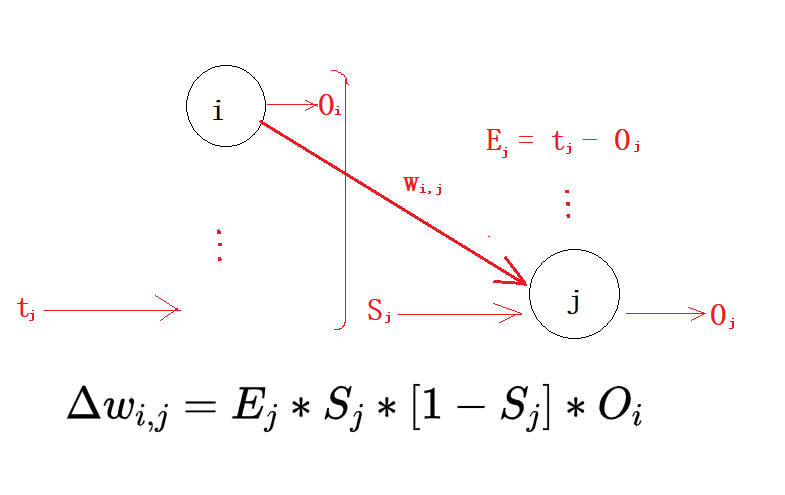
\includegraphics[scale=0.3]{picture/公式参数.png}
        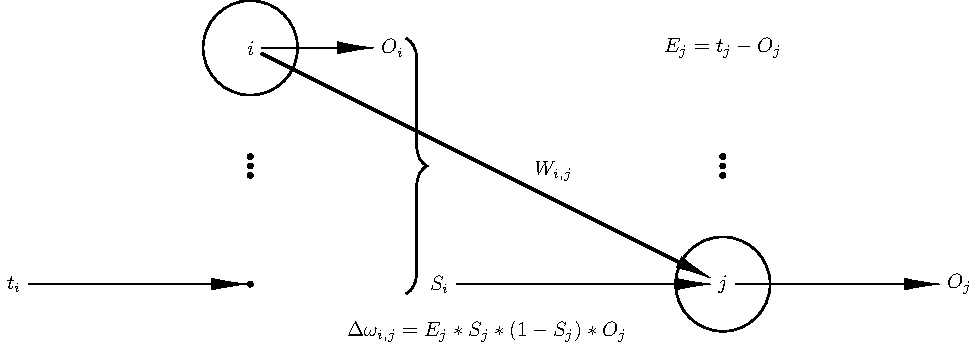
\includegraphics[scale=0.7]{picture/coef_distrio.pdf}
    \end{figure}
    \newpage
    一个具体的实例计算:
    \begin{align}
        \Delta w_{2,1} 
        & = \frac{\partial E}{\partial w_{2,1}} \nonumber \\
        & =-e_1\cdot {\rm sigmoid}(i'_1)\cdot [1-{\rm sigmoid}(i'_1)]\cdot O_2 \nonumber\\
        &  = E_1*S_1(1-S_1)\cdot O_2 \nonumber
    \end{align}
    我们把所有的权重考虑进来,就可以把所有的权重调整计算转化为矩阵的运算
    这一过程的矩阵图解如下:
    \begin{equation}
            \begin{bmatrix}
                \Delta w_{1,1} & \Delta w_{2,1} & \Delta w_{3,1} & \cdots\\
                \Delta w_{1,2} & \Delta w_{2,2} & \Delta w_{3,2} & \cdots\\
                \Delta w_{1,3} & \Delta w_{2,3} & \Delta w_{j,k} & \cdots \\
                \cdots         & \cdots         & \cdots         & \cdots
            \end{bmatrix}
                =
            \begin{bmatrix}
                E_{1} * S_{1}\left(1-S_{1}\right) \\
                E_{2} * S_{2}\left(1-S_{2}\right) \\
                E_{3} * S_{3}\left(1-S_{3}\right) \\
                \cdots 
            \end{bmatrix}
                \cdot 
            \begin{bmatrix}  
                O_1,O_2,\cdots ,O_n
            \end{bmatrix}
    \end{equation}
    
    由于学习率只是一个常数, 并没有真正改变如何组织矩阵乘法, 因此由于学习率只是一个常数,并没有真正改变如何组织
    矩阵乘法,因此我们省略了学习率$\alpha$。我们省略了学习率$\alpha$。上面等式右边的第一项即为下一层的值,
    第二项为前一层的值,等式的左边为权重变化矩阵。

    权重变化矩阵中包含了诸多的值, 这些值可以调整链接权重$w_{j,k}$,这个权重链接了
    当前层节点j与下一层节点k。你可以发现, 表达式中的第一项使用下一层(k层)
    的输出值, 最后一项使用前一层(j层)的输出值。
    仔细观察上面, 你就会发现,表达式的最后一部分,也就是单行的水平矩阵,是前一层$O_j$
    的输出的转置。如果你不能确定, 可以尝试使用另一种方式的点乘, 
    你会发现这是行不通的。因此, 权重更新矩阵有如下的矩阵形式, 这种形式可以让我们通过计算机编程语言高效地
    实现矩阵运算。
    
    最终的权重计算公式即为
    \begin{equation}
        \boxed
        {
        \Delta W_{j, k}=\alpha * E_{k} * S_{k}\left(1-S_{k}\right) \cdot O_{j}^{T}
        }
    \end{equation}
    
    \textbf{注:*是普通乘法,$\cdot$ 是矩阵乘法。}

    \clearpage
    关于误差矩阵的可视化我们采用如下的方式,误差矩阵参数分布的示意图如下:
    \begin{figure}[!htb]
        \centering
        % 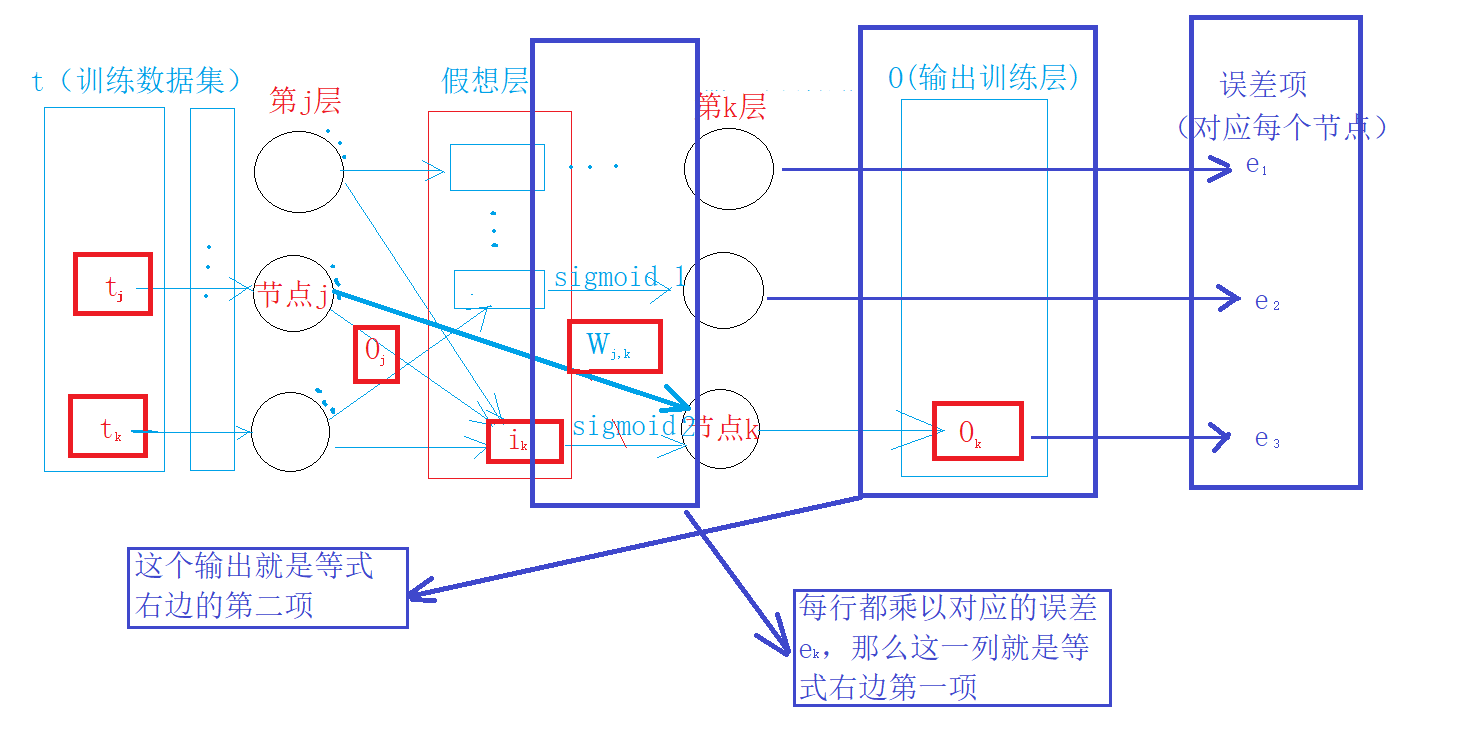
\includegraphics[scale=0.5]{picture/误差矩阵参数分布.png}
        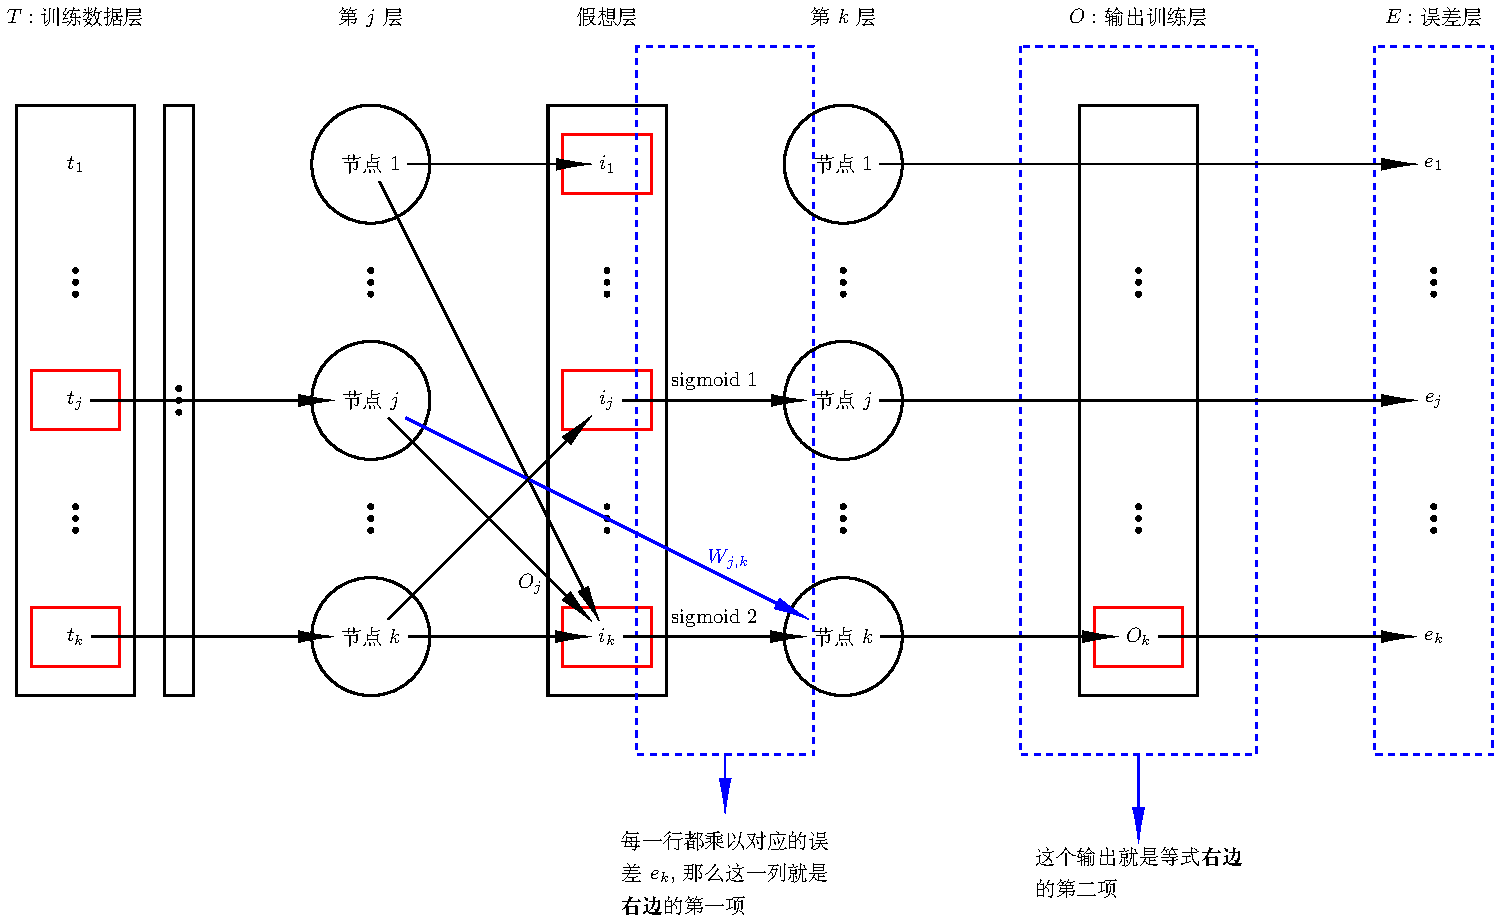
\includegraphics[scale=.5]{./picture/coef.pdf}
        \caption{误差矩阵参数分布}
    \end{figure}

    可以这样理解:$w_{j,k}$中,j是神经网络的第j列,k是第k行
   
    % \clearpage
    \subsection{权重更新的范例}
    下边我们给出一个实例:
    \begin{figure}[!htb]
        \centering
        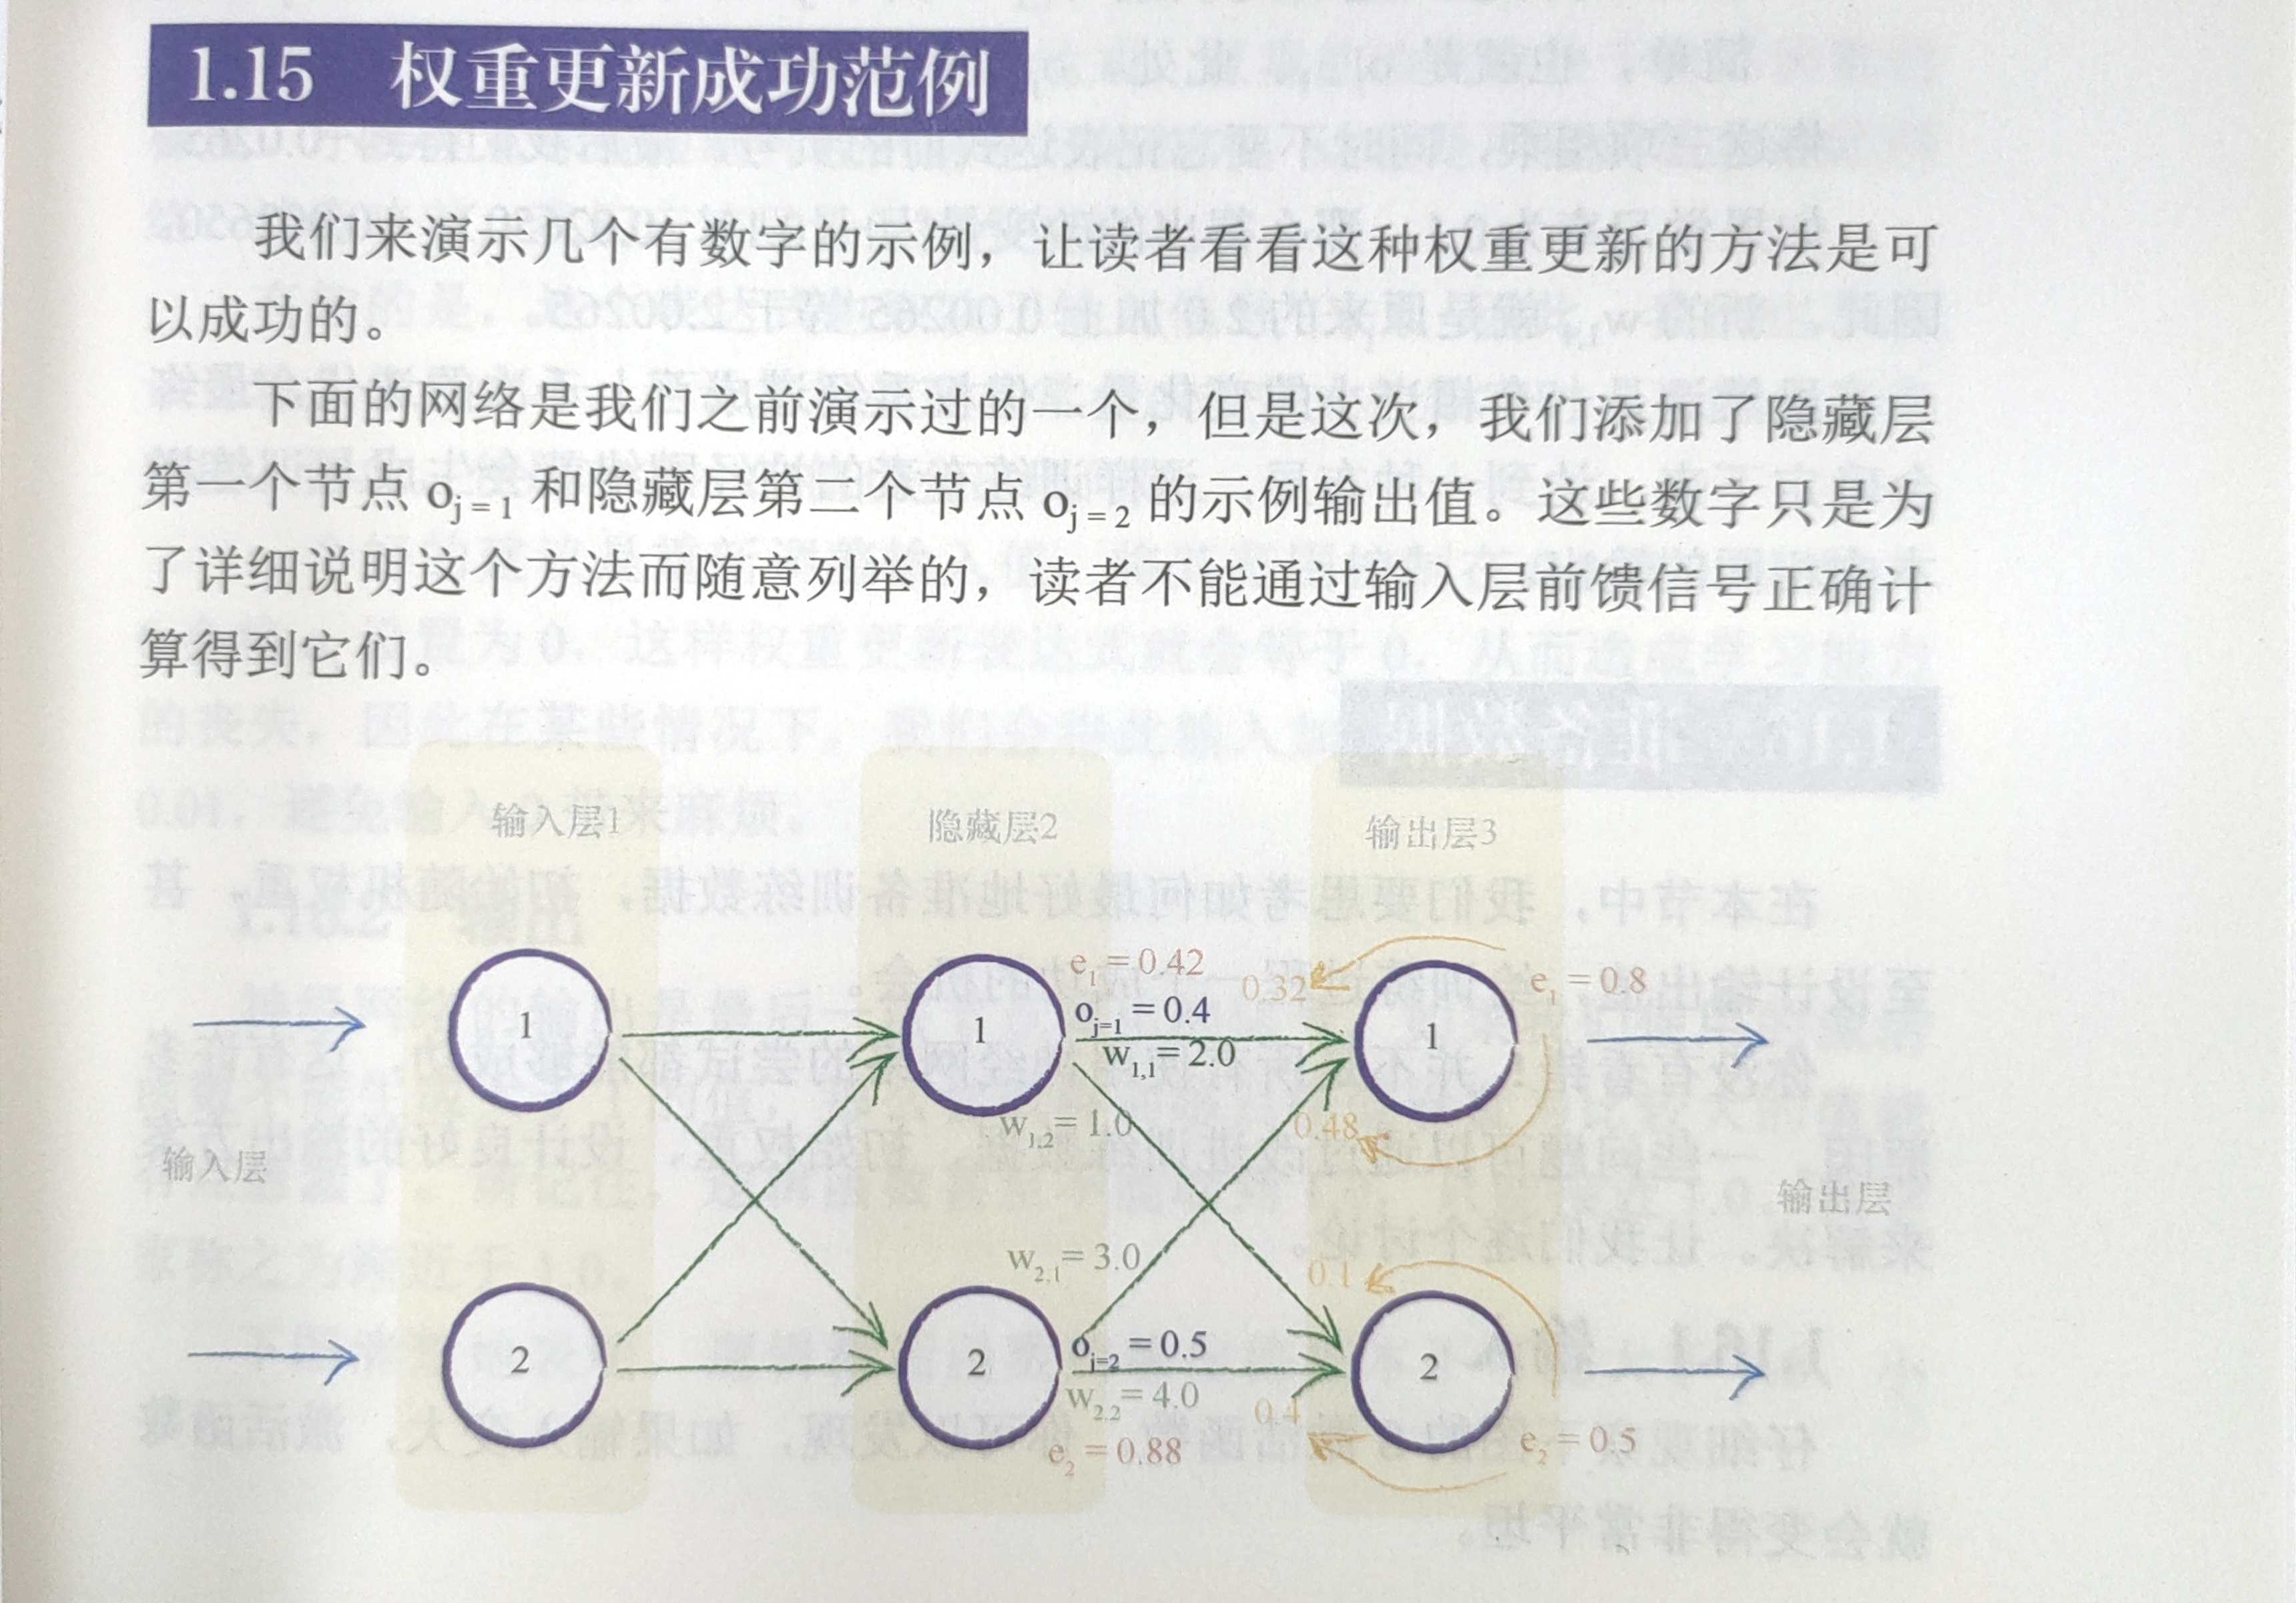
\includegraphics[scale=0.1]{picture/实例1.jpg}
    \end{figure}
    \begin{figure}[!htb]
        \centering
        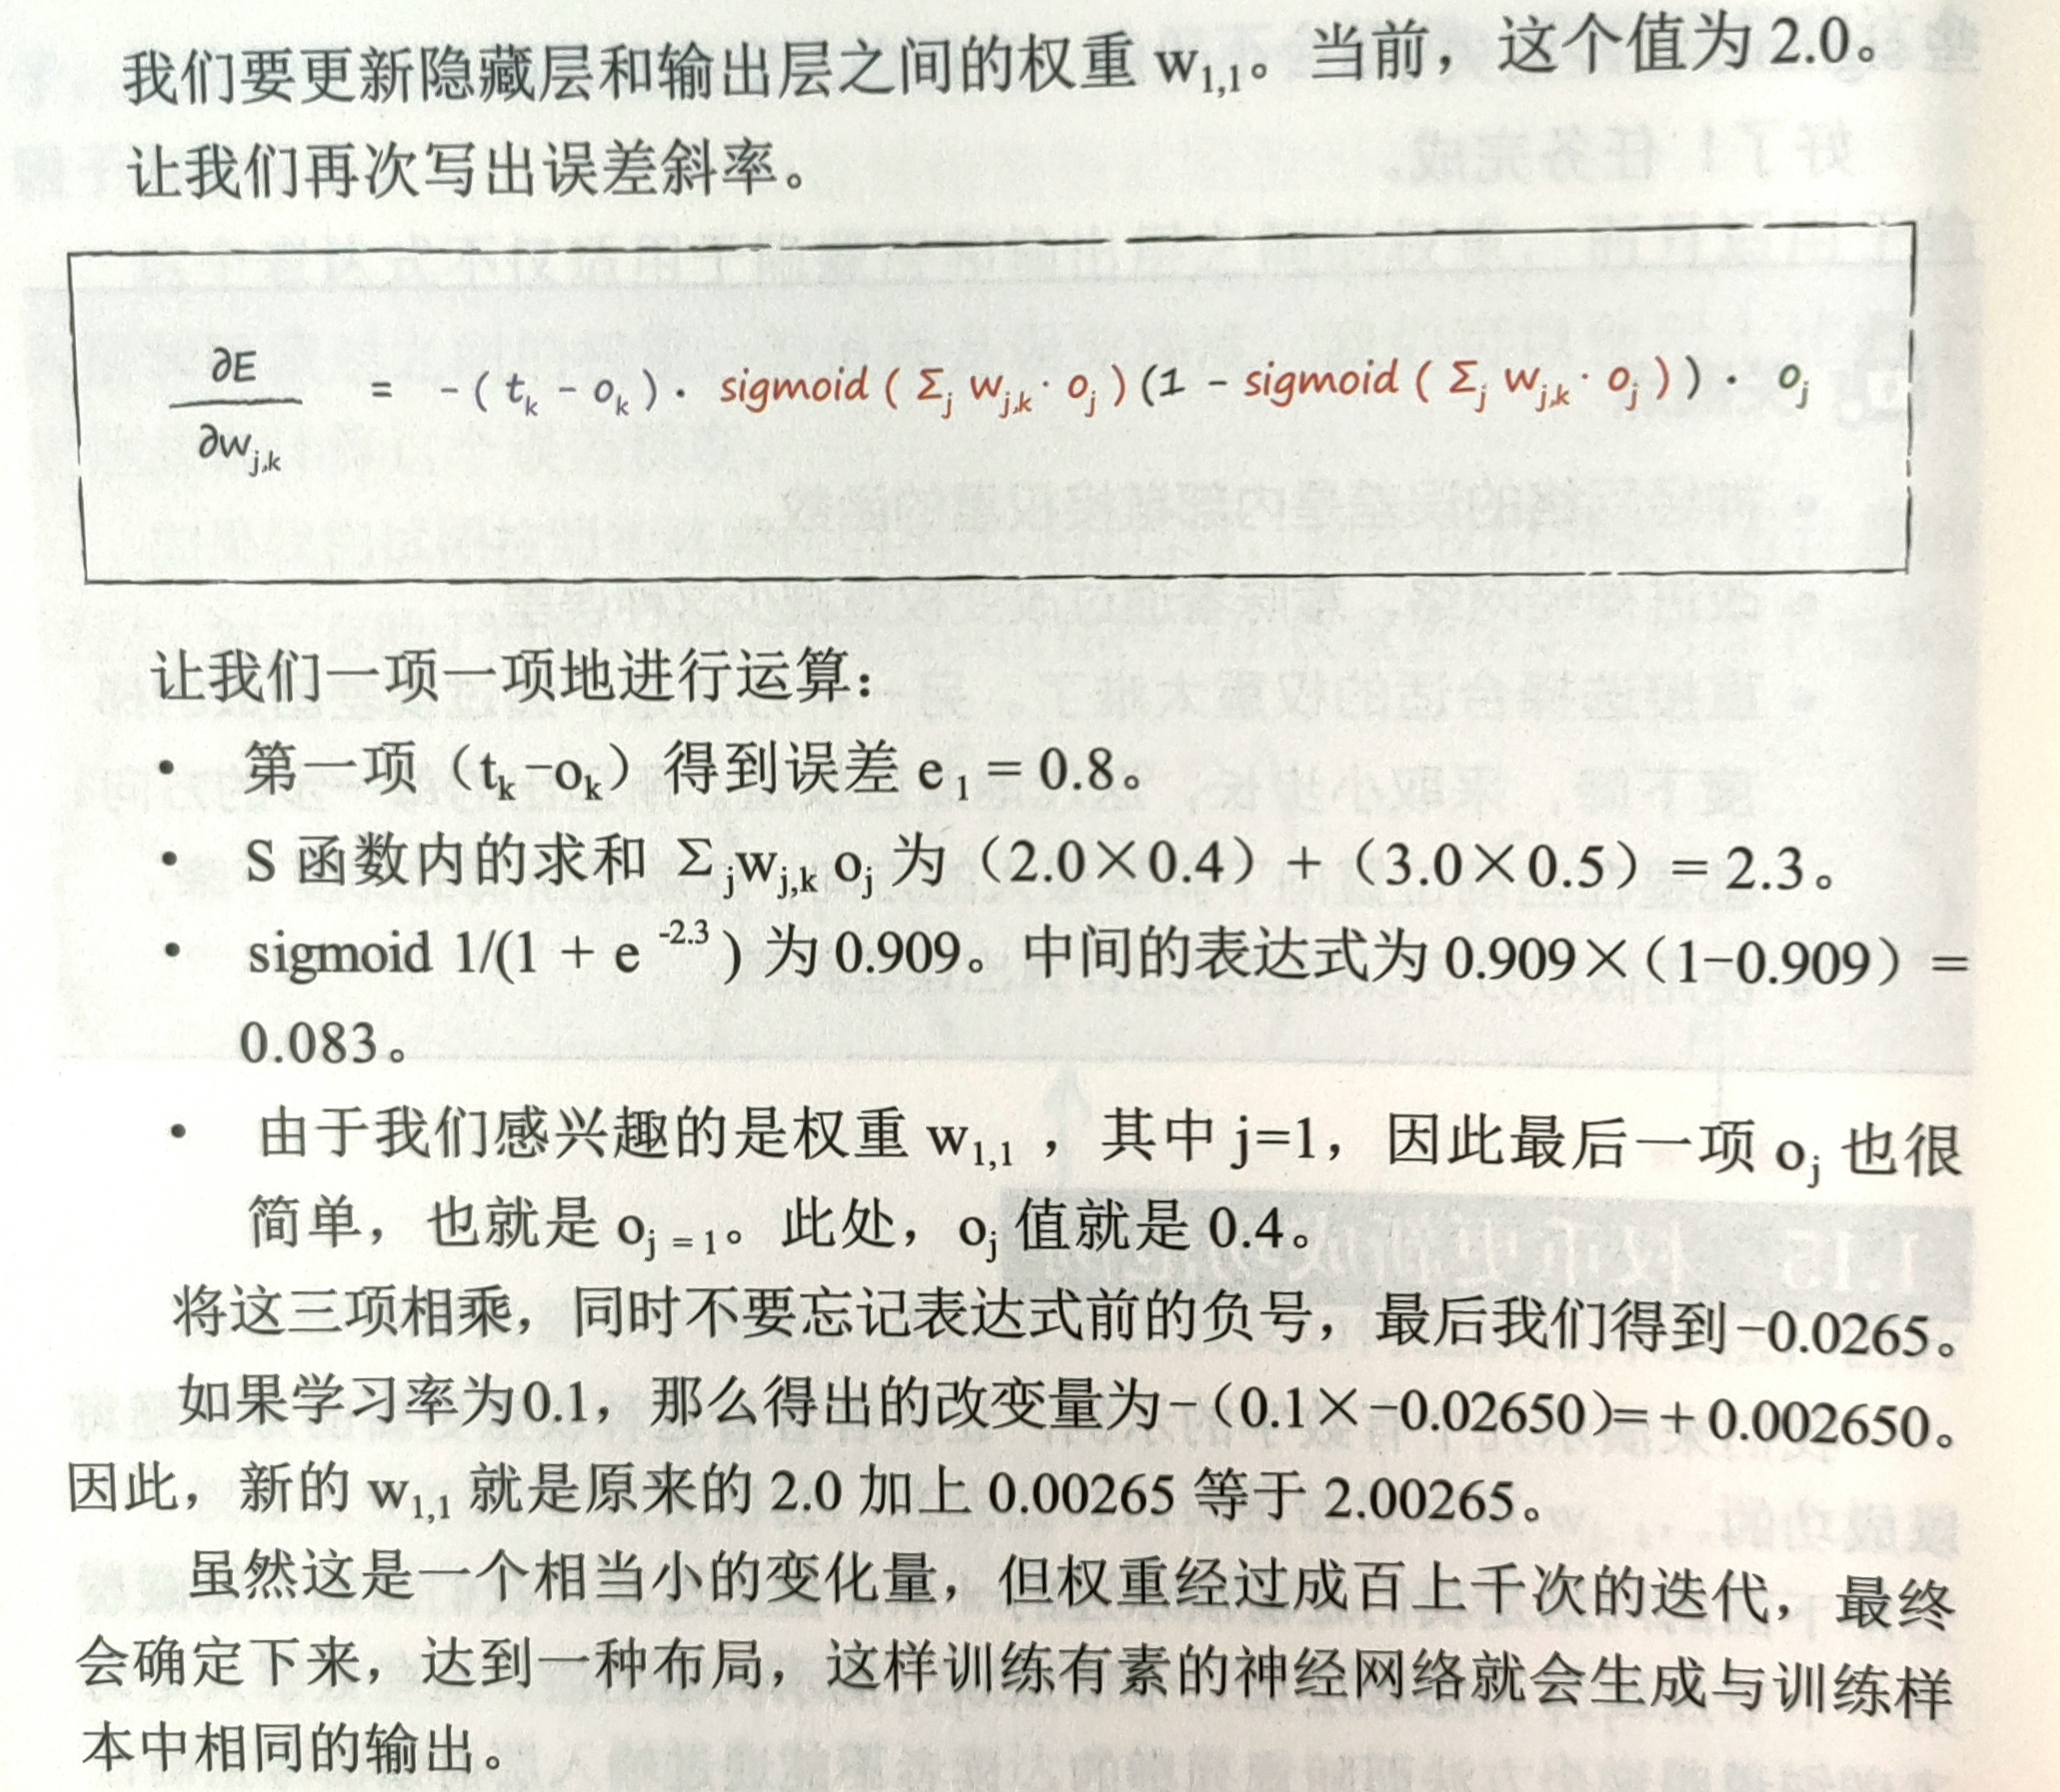
\includegraphics[scale=0.12]{picture/实例2.jpg}
        \label{实例}
    \end{figure}
    
    \subsection{准备数据}
    在本节里边我们会思考如下的问题
    \begin{itemize}
        \item 如何准备训练数据
        \item 如何初始化权重
        \item 如何设计输出值
    \end{itemize}

    $\S1$训练数据\\
    因为我们采用的是梯度学习新的权重,也就是说权重的改变取决于激活函数的梯度。
    但是sigmoid函数在x很大时,变化很慢,这样的结果就是:限制神经网络的学习能力,造成\textbf{饱和神经网络}。
    这就意味着我们必须要保证较小的输入,防止饱和。我们还可以得出,梯度改变与$O_i$,也就是输入数据有关。
    所以输入数据$O_i$不能等于0,一旦等于0,那么$\Delta w_{i,j}=0$,神经网络就丧失了学习能力。
    
    $\S2$目标值设定\\
    因为$S(x)\in (0,1)$,所以我们的训练目标值不能够过大,也就是说我们的目标值很大的话,
    网络会驱使生成较大的权重,来获得大的输出。这时网路的权重较大,传递给激活函数的信号(值)过强,
    神经网络就会达到饱和。所以常用的范围是:$R = [0.01,0.99]$

    $\S3$权重初始化\\
    从$\S2$我们也可以明白,权重不易过大。但是我们并不一定是从$(-1,1)$这个大范围内随机选取权重。
    对于给定的神经网络和激活函数,我们有更好的方案。

    但是我们有一个核心思想:如果有一些很好(不太大,分布较为均匀,)的信号进入了一个节点,
    那么权重应该包持这些信号不变,也就是说,和这些信号相关的权重尽量维持稳定。
    我们有一条经验规律:加入每个节点有N条传入链接,那么这些链接上边的权重就应该在$(-\frac{1}{\sqrt{N}},\frac{1}{\sqrt{N}})$
    范围内选取。直观理解就是:如果一个节点的传入链接过多,那么它们的和就可能比较大或者是存在较大的权重在里边,导致它们的和较大,
    因此我们限制权重的范围在小一点的范围就可以解决这个问题。

    \section{实践编程}
    \vspace{12em}
    \begin{center}
        \Huge
        $\mathscr{T}he\qquad \mathscr{E}nd$
    \end{center}


    





\end{document}

